\PassOptionsToPackage{table}{xcolor}
\documentclass[12pt,letterpaper,twocolumn,openany,nodeprecatedcode,bg=none]{dndbook}
\usepackage[english]{babel}
\usepackage[utf8]{inputenc}
\usepackage{longtable,booktabs,array}
\usepackage{calc}
\usepackage{etoolbox}
\usepackage{caption}
\usepackage{float}
\usepackage{graphicx}
\usepackage{needspace}
\usepackage{tikz}

% Reset zebra striping at the start of every table
\AtBeginEnvironment{longtable}{\rowcolors{1}{white}{gray!10}\small}
\AtBeginEnvironment{table}{\rowcolors{1}{white}{gray!10}}

\providecommand{\pandocbounded}[1]{#1}
\providecommand{\tightlist}{%
  \setlength{\itemsep}{0pt}\setlength{\parskip}{0pt}}

\captionsetup{labelformat=empty}
\setcounter{secnumdepth}{0}
\setlength{\parindent}{0pt}
\setlength{\parskip}{0.5\baselineskip}
\setlength{\headheight}{15pt}

% Prevent orphaned subsections
\let\oldsubsection\subsection
\renewcommand{\subsection}[1]{%
  \needspace{5\baselineskip}%
  \oldsubsection{#1}%
}

\begin{document}
\onecolumn

      \title{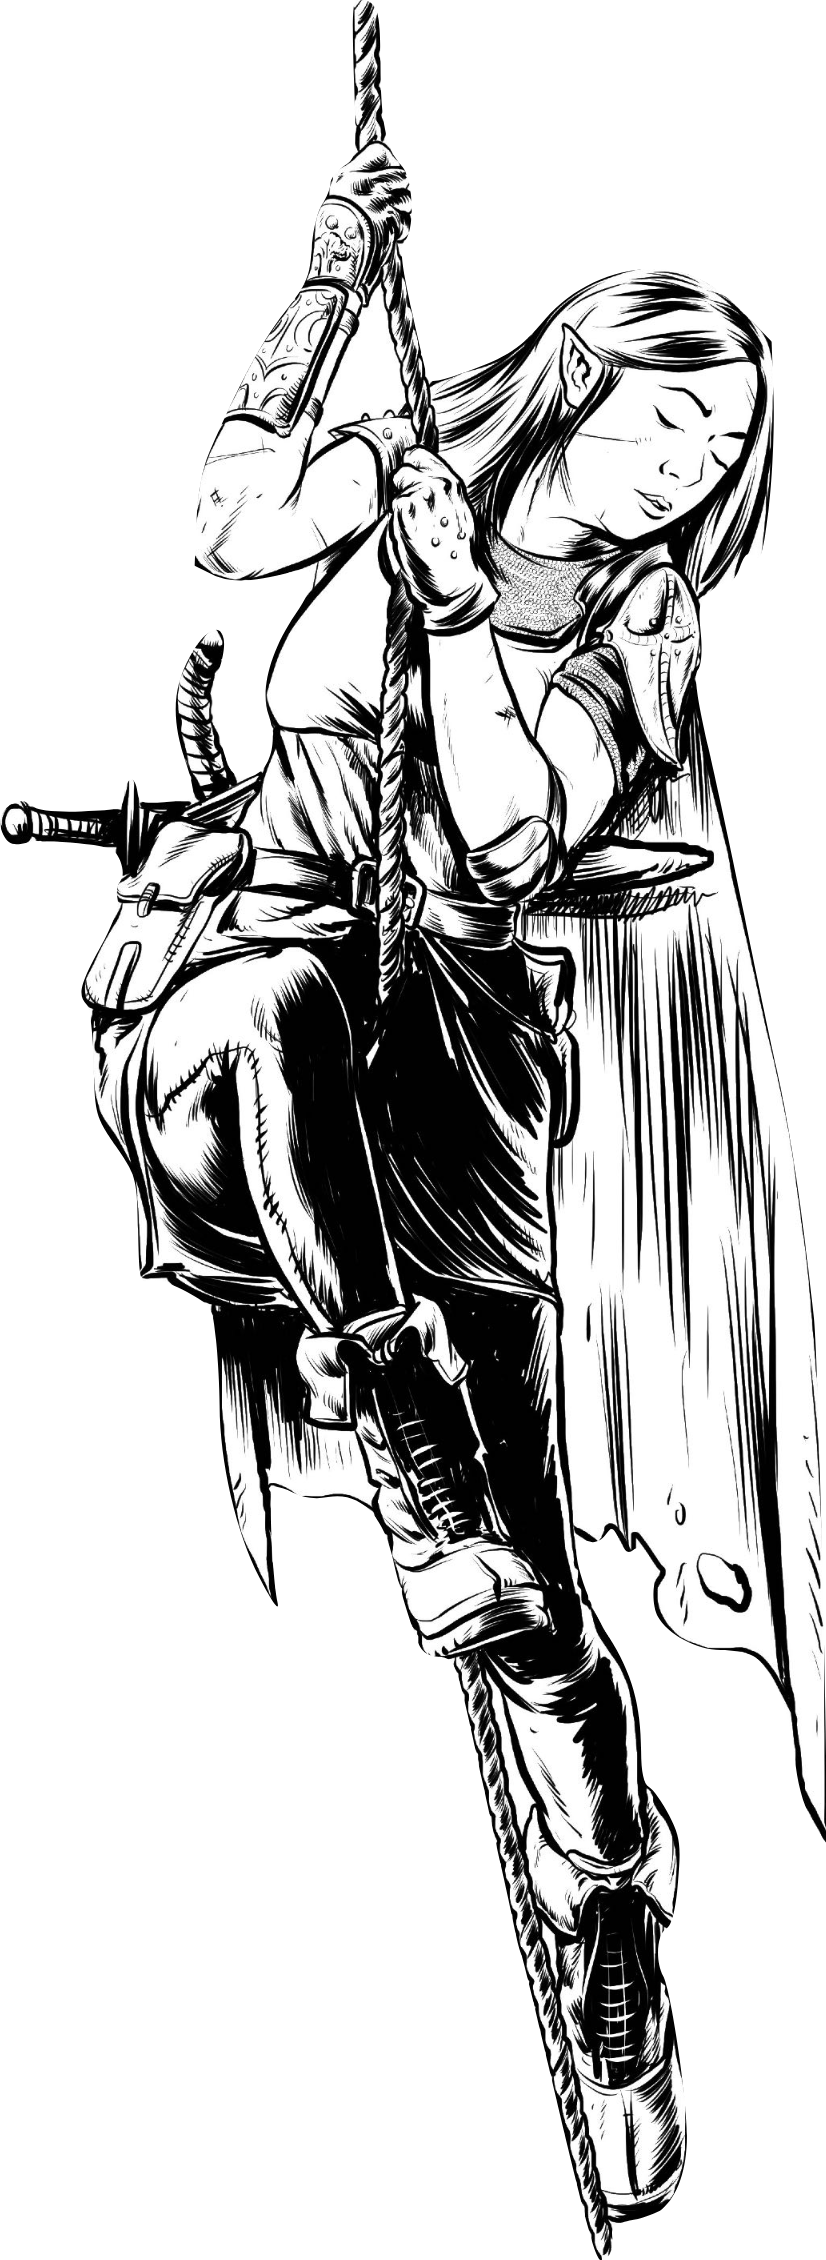
\includegraphics[width=0.9\textwidth,height=0.55\textheight,keepaspectratio]{femaleRogue.png}\\[1.5cm]Rogue}
  \author{Class Handbook}
\date{}
\maketitle

\clearpage
\thispagestyle{empty}
\null\vfill
\begin{center}{\Large\itshape Your trusty class handbook for fantasy
gaming.}\end{center}
\vfill

\clearpage
\thispagestyle{empty}
\begin{center}
\vspace*{\fill}
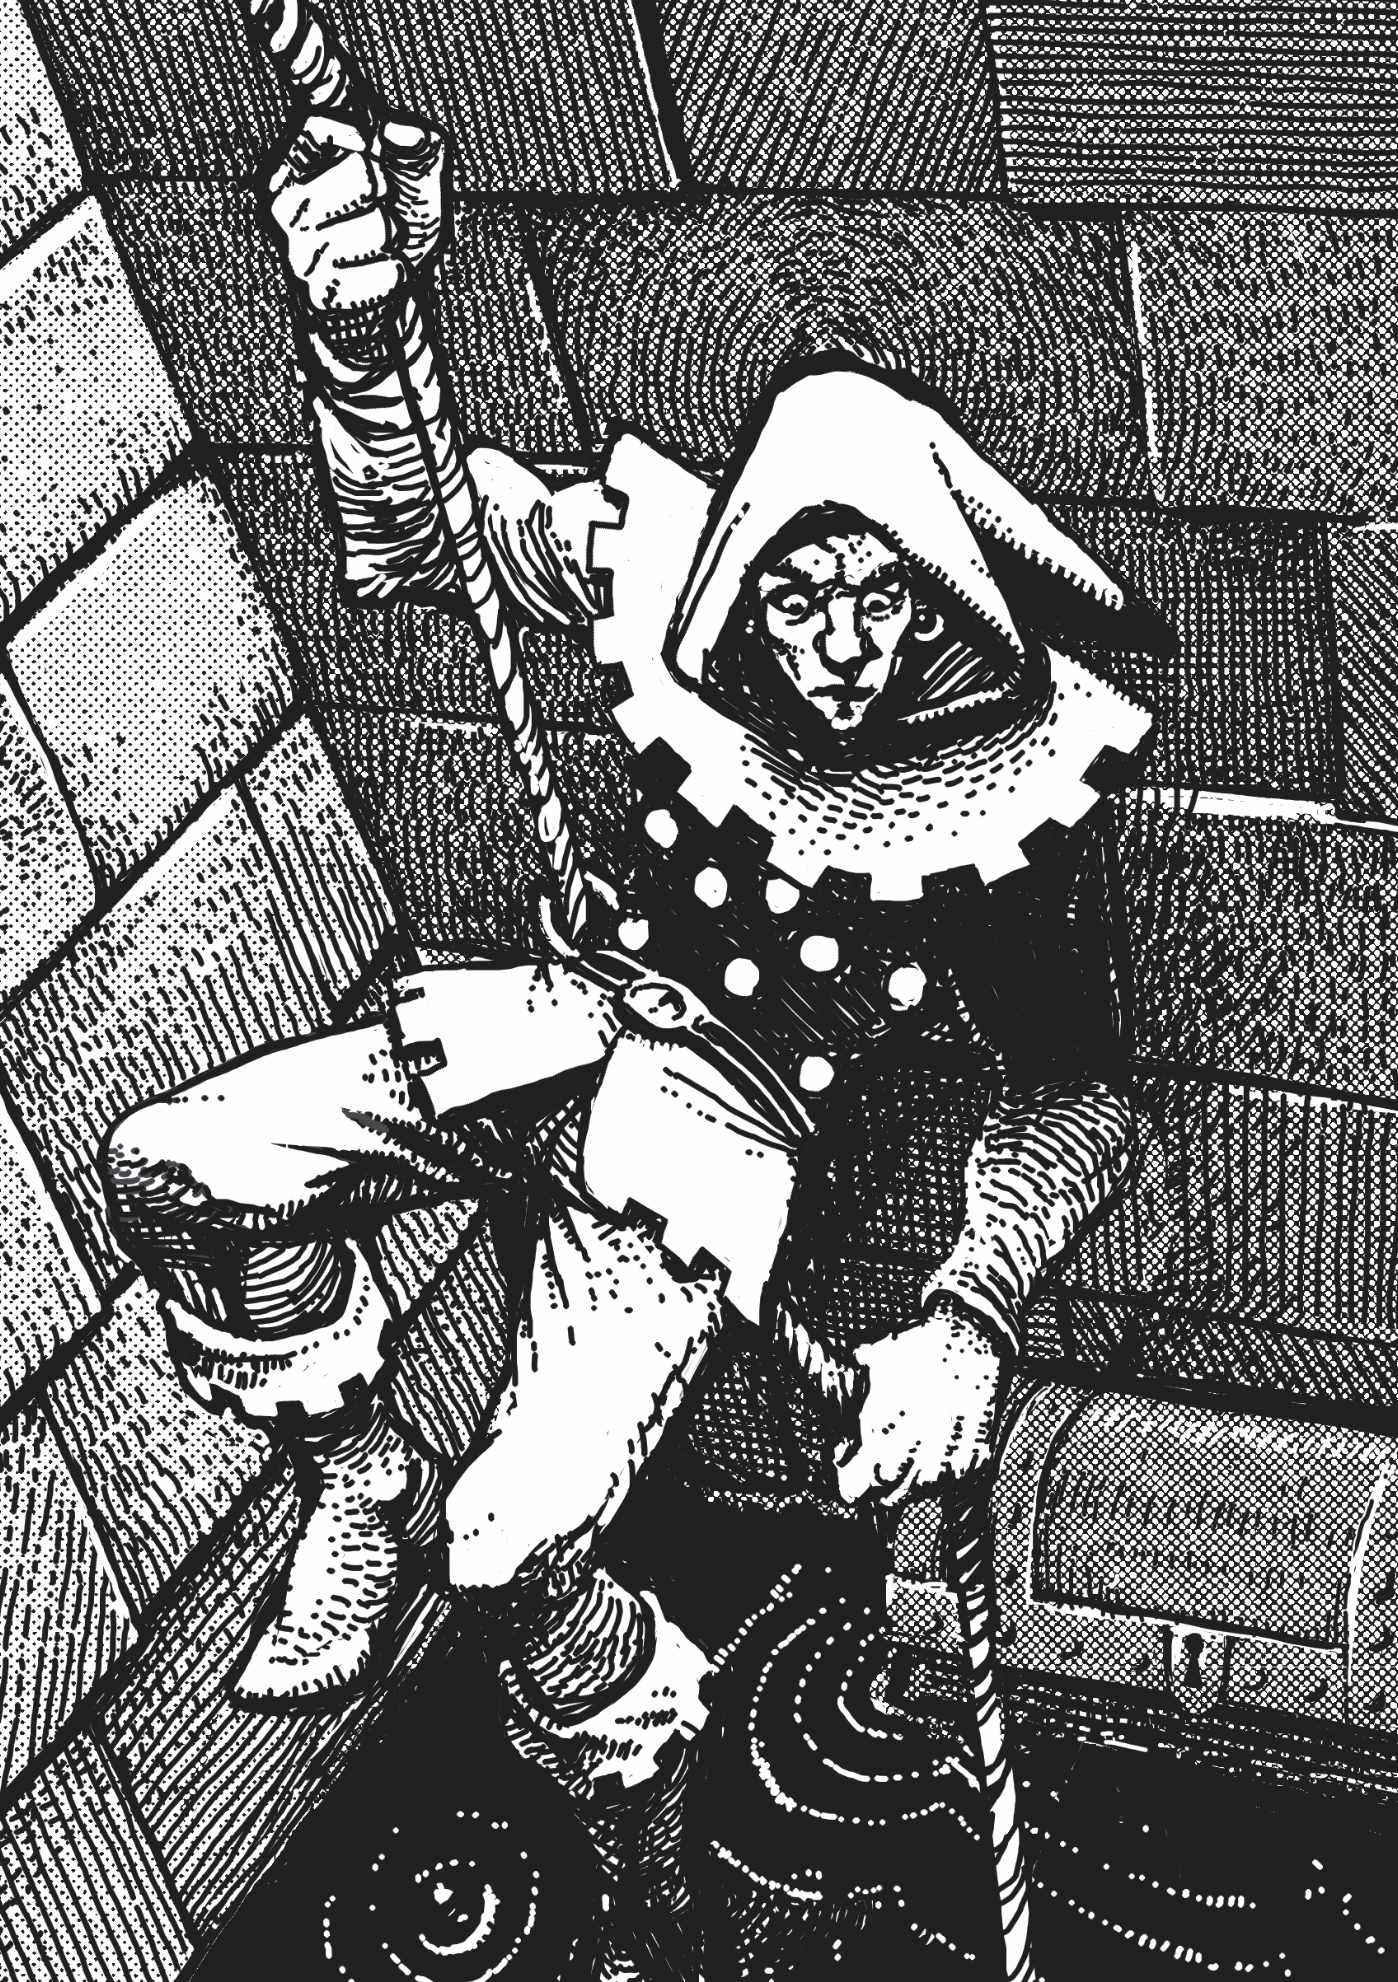
\includegraphics[width=\textwidth,height=0.85\textheight,keepaspectratio]{thiefSD.png}\par
\vspace{0.4cm}
{\itshape A rogue drops into action}\par
\vspace*{\fill}
\end{center}

\clearpage
\twocolumn

\onecolumn

\section{Rogue}\label{rogue}

\subsection{Core Rogue Traits}\label{core-rogue-traits}

\needspace{11\baselineskip}

{\def\LTcaptype{none} % do not increment counter
\begin{table}[!htbp]
\centering
\begin{tabular}{@{}
  >{\raggedright\arraybackslash}p{(\linewidth - 2\tabcolsep) * \real{0.3171}}
  >{\raggedright\arraybackslash}p{(\linewidth - 2\tabcolsep) * \real{0.6829}}@{}}
\toprule\noalign{}
\begin{minipage}[b]{\linewidth}\raggedright
\textbf{Primary Ability}
\end{minipage} & \begin{minipage}[b]{\linewidth}\raggedright
Dexterity
\end{minipage} \\
\midrule\noalign{}
\textbf{Hit Points} & 1d4 \\
\textbf{Saving Throw Proficiencies} & Dexterity, Intelligence \\
\textbf{Skill Proficiencies} & Choose 4 skills \\
\textbf{Weapon Proficiencies} & Choose 3 categories \\
\textbf{Starting Equipment} & Padded Jacket, Cloak, 2 Daggers, Sabre,
Thieves' Tools \\
\bottomrule\noalign{}
\end{tabular}
\end{table}
}

\subsection{Rogue Features}\label{rogue-features}

\needspace{20\baselineskip}

{\def\LTcaptype{none} % do not increment counter
\begin{table}[!htbp]
\centering
\begin{tabular}{@{}
  >{\raggedright\arraybackslash}p{(\linewidth - 4\tabcolsep) * \real{0.1064}}
  >{\raggedright\arraybackslash}p{(\linewidth - 4\tabcolsep) * \real{0.2340}}
  >{\raggedright\arraybackslash}p{(\linewidth - 4\tabcolsep) * \real{0.6596}}@{}}
\toprule\noalign{}
\begin{minipage}[b]{\linewidth}\raggedright
Level
\end{minipage} & \begin{minipage}[b]{\linewidth}\raggedright
Proficiency
\end{minipage} & \begin{minipage}[b]{\linewidth}\raggedright
Class Features
\end{minipage} \\
\midrule\noalign{}
1 & +2 & Sneak Attack, Roguish Archetype \\
2 & +2 & --- \\
3 & +2 & Cunning Action, Ability Bonus \\
4 & +2 & --- \\
5 & +2 & --- \\
6 & +2 & --- \\
7 & +2 & Ability Bonus \\
8 & +2 & --- \\
9 & +3 & Uncanny Dodge \\
10 & +3 & --- \\
\bottomrule\noalign{}
\end{tabular}
\end{table}
}

\subsection{Level 1: Sneak Attack}\label{level-1-sneak-attack}

You deal 1d6 extra damage with weapons if you have advantage on your
attack roll or if the target is in melee range of a creature friendly to
you.

This damage increases to 2d6 at level 3, 3d6 at level 5, and 4d6 at
level 7. At level 9, the rogue has become a master of finding a foe's
weak points, the damage jumps to 5d10.

\twocolumn

\subsection{Level 1: Roguish Archetype}\label{level-1-roguish-archetype}

All rogues have a specialty, a focus for their activities that defines
their career. Pick one of the following options. Each one gives you a
special set of abilities.

\begin{itemize}
\tightlist
\item
  \textbf{Acrobat.} You gain a climb speed. You take no damage from
  falling. You can walk across surfaces as narrow as one inch, such as a
  rope.
\item
  \textbf{Arcane Trickster.} You gain an illusionist cantrip of your
  choice and can cast one illusionist spell once per long rest. Each
  time you gain a level, you can swap those choices for different
  options. You use the rules for casting spells as per the illusionist
  class.
\item
  \textbf{Assassin.} You are a hired killer capable of felling even the
  mightiest opponent with a single blow. You gain your Intelligence
  modifier as a bonus to damage rolls. As a search action, you can study
  a target within 30 feet. On your next turn, roll double the number of
  sneak attack dice you normally roll.
\item
  \textbf{Bardic Apprentice.} You know how to play two musical
  instruments and gain proficiency with the performance skill, you gain
  expertise if you are already proficient with that skill. You can
  figure out how to use magic items that would otherwise require
  class-specific knowledge.
\item
  \textbf{Brawler.} You gain an additional weapon proficiency and reduce
  the strength requirement for armor you wear by 1.
\item
  \textbf{Con Artist.} You excel at adopting various disguises and
  personas to win trust. You have advantage on all checks made to
  convince others that you are a long lost friend, comrade, or member of
  their organization.
\item
  \textbf{Pirate.} You gain an additional weapon proficiency and a swim
  speed. You know how to navigate by the constellations.
\item
  \textbf{Scout.} You gain an additional weapon proficiency and
  proficiency with the Nature and Survival skills. If you are already
  proficient with a skill gained from this feature, you gain expertise
  with it. You also know how to navigate by the constellations.
\item
  \textbf{Thief.} You gain a bonus to Stealth checks equal to your
  Intelligence modifier. If you are hidden and do anything on your turn
  to reveal yourself, you can try to hide again that turn. Normally when
  you reveal yourself you cannot try to hide again.
\end{itemize}

\subsection{Level 3: Cunning Action}\label{level-3-cunning-action}

Once on your turn, you can dash, disengage, or hide without using your
action.

\subsection{Level 3: Ability Bonus}\label{level-3-ability-bonus}

You gain a +1 bonus to two different abilities of your choice.

\subsection{Level 7: Ability Bonus}\label{level-7-ability-bonus}

You gain a +1 bonus to two different abilities of your choice.

\subsection{Level 9: Uncanny Dodge}\label{level-9-uncanny-dodge}

You halve the damage you take from a single attack or effect. Once you
use this feature, you can't use it again until your next turn.

\onecolumn

\begin{figure}
\centering
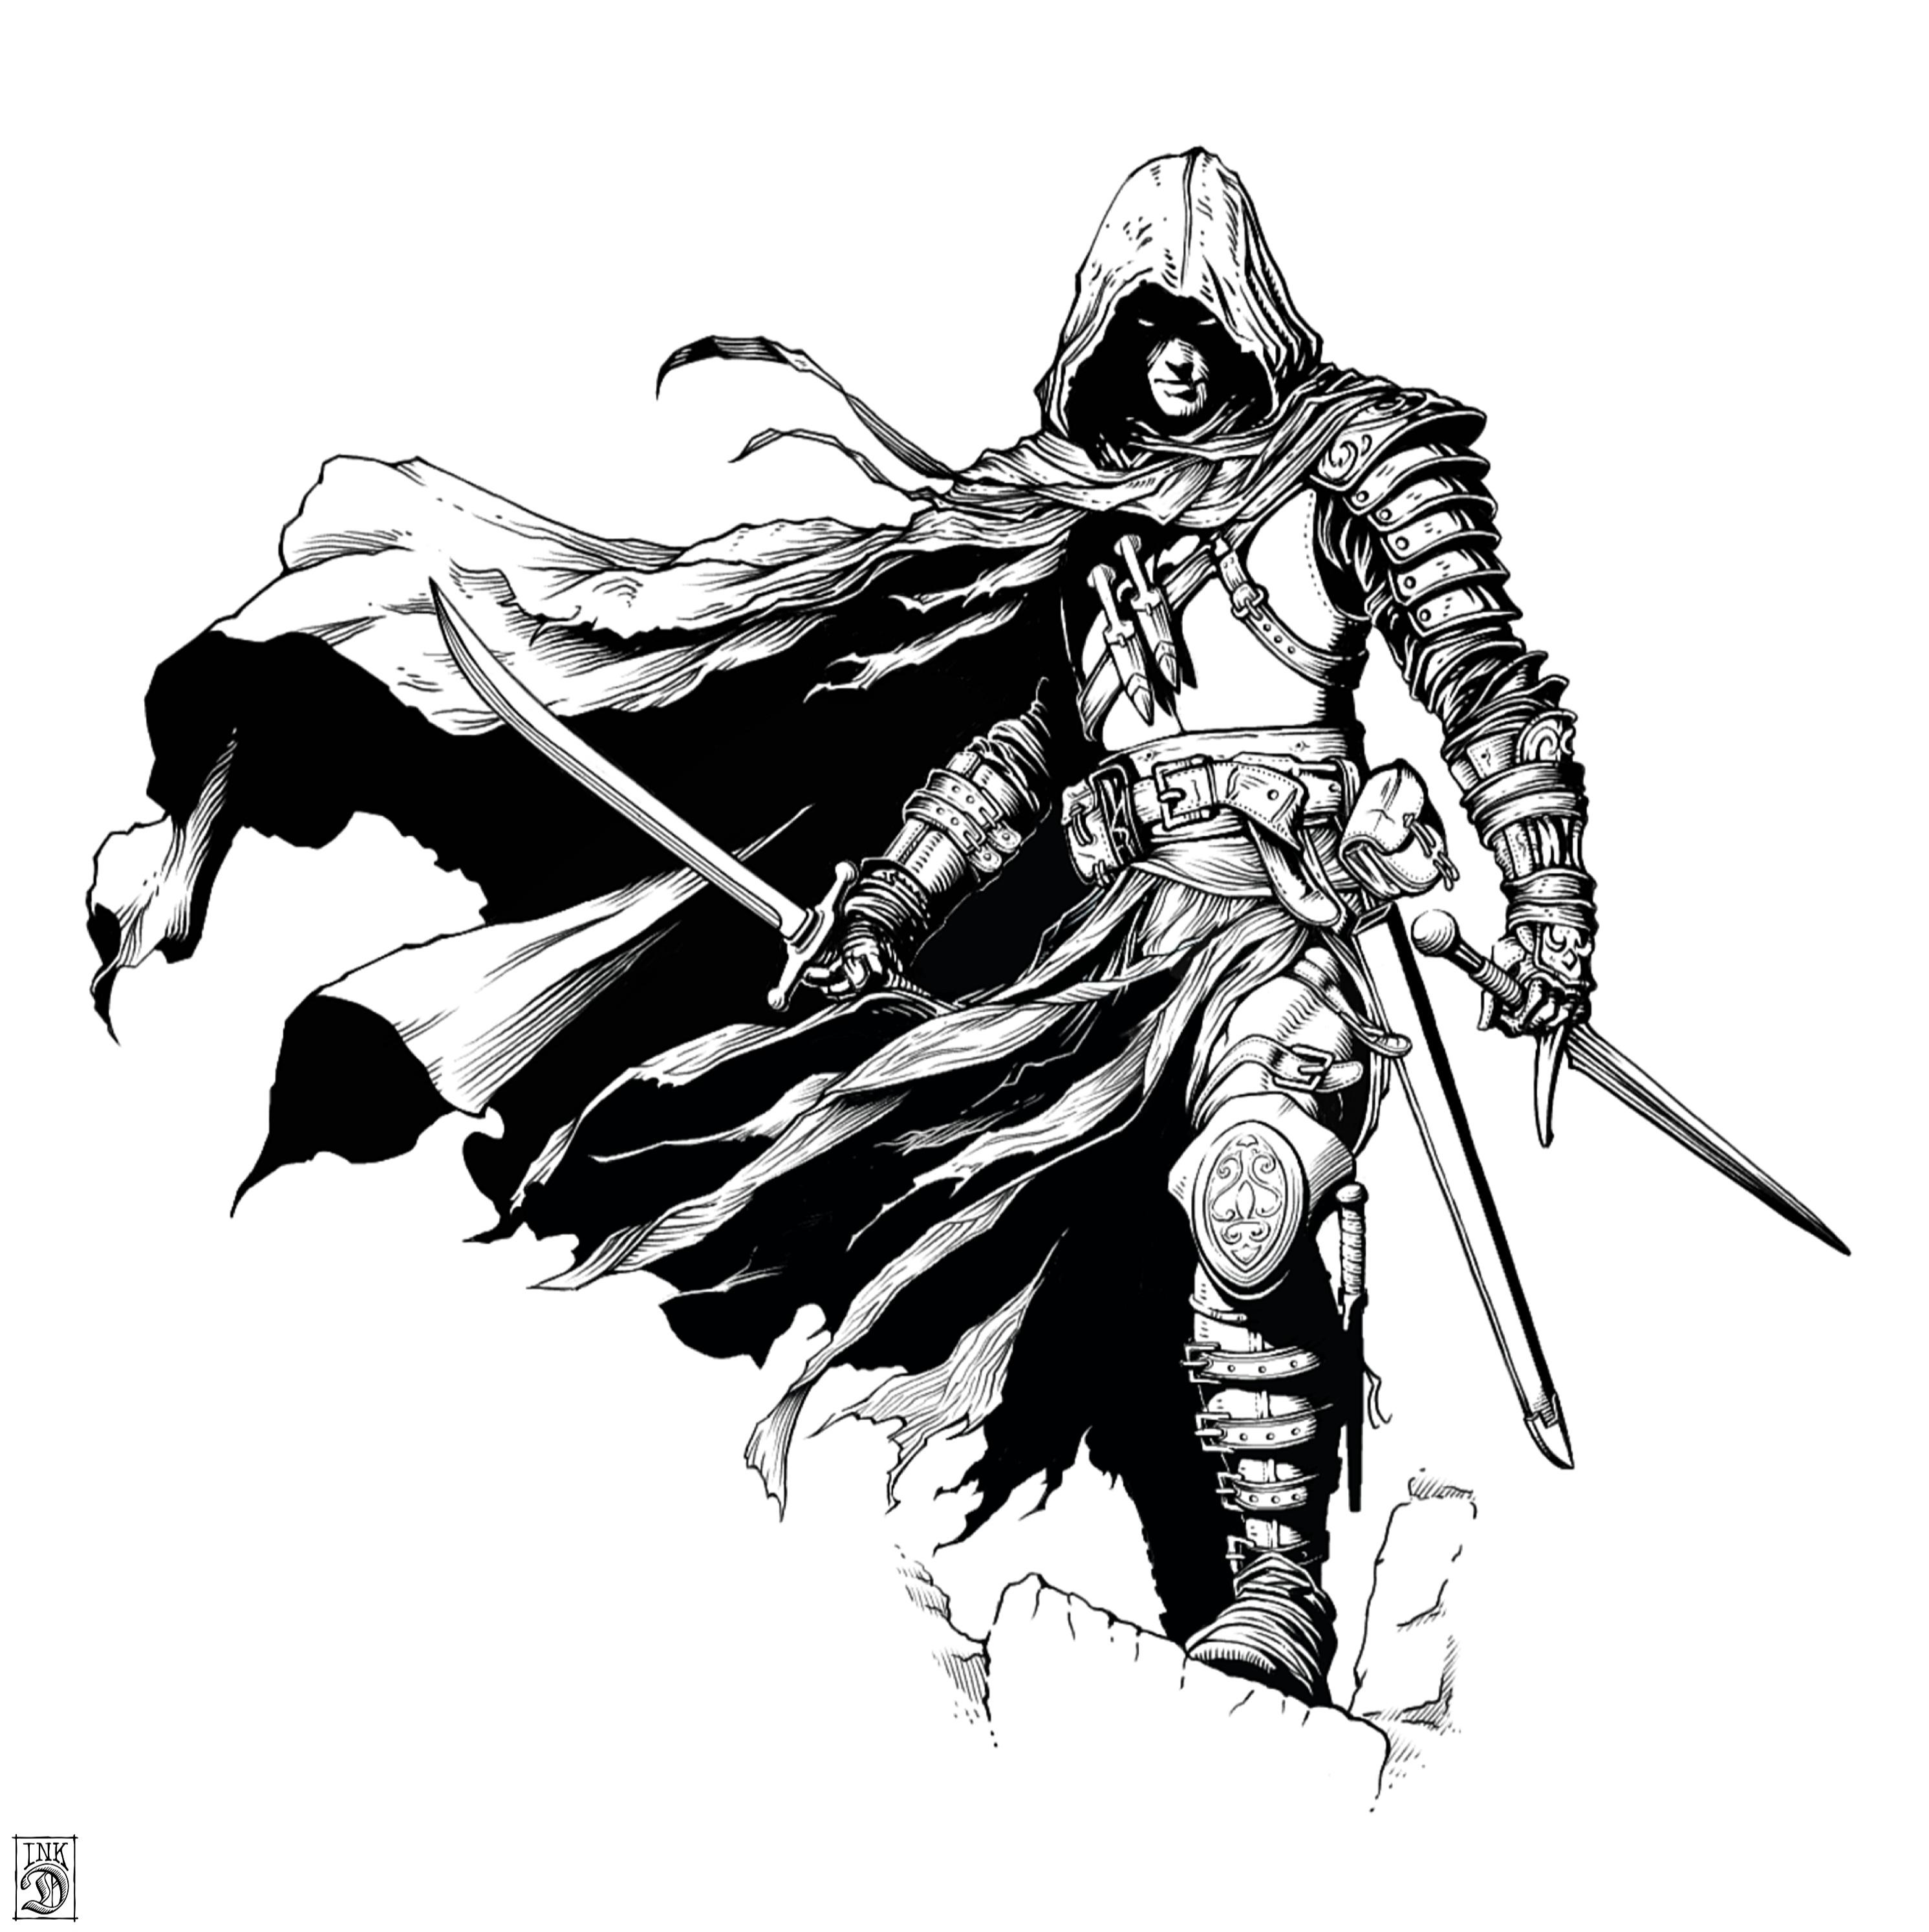
\includegraphics[width=0.9\linewidth,height=\textheight,keepaspectratio,alt={A
classic edge-lord}]{classicEdgelord.jpeg}
\caption{A classic edge-lord}
\end{figure}

\clearpage

\begin{center}

\begin{figure}
\centering
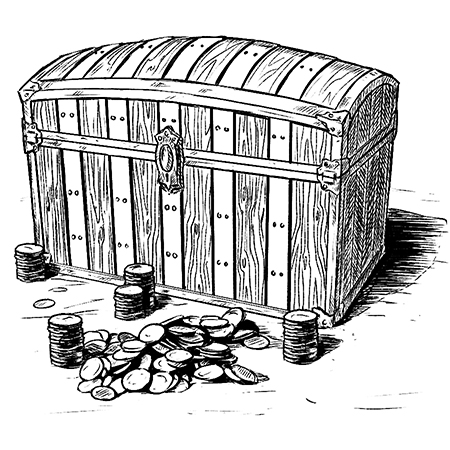
\includegraphics[width=0.9\linewidth,height=\textheight,keepaspectratio,alt={Look
at all that gold\ldots{}}]{treasureChest.jpg}
\caption{Look at all that gold\ldots{}}
\end{figure}

\end{center}

\onecolumn

\clearpage
\thispagestyle{empty}
\begin{center}
\vspace*{\fill}
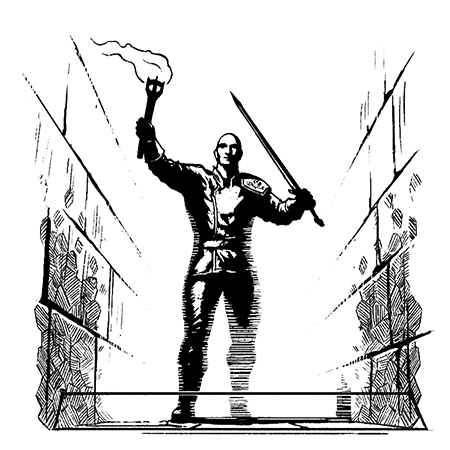
\includegraphics[width=0.7\textwidth,keepaspectratio]{adventurerShadows.jpg}\par
\vspace{0.4cm}
{\itshape Rogues make great dungeon delvers}\par
\vspace*{\fill}
\end{center}

\end{document}